\documentclass[10pt, a4paper]{article}
\usepackage[top=60pt, bottom=50pt, left=72pt, right=55pt]{geometry}
\usepackage{enumerate}
\usepackage[fleqn]{amsmath}
\usepackage{amssymb}
\usepackage{graphicx}
\begin{document}
	\title{PH-105 Assignment Sheet - 2 (Quantum Mechanics)}
	\date{}
	\author{Umang Mathur}
	\maketitle
	\begin{enumerate}
		\item[10.] {\bf A photon of energy $h\nu$ is scattered through 90$^{\circ}$ by an electron initially at rest. The scattered photon has a wavelength twice that of incident photon. Find the frequency of the incident photon and the recoil angle of the electron.}\\\\
		{\underline {\bf Solution}} :\\
		
		In Compton Scattering, the relation between the final wavelength ($\lambda'$) and the intial wavelength ($\lambda$) is given by:
		\begin{align*}
			\lambda' - \lambda = \frac{h}{m_{o}c}(1-\cos\theta)
		\end{align*}
		Given that $\lambda' = 2\lambda$ and $\theta = 90^{\circ}$, we have $\lambda = \frac{h}{m_{o}c}$.\\
		Hence, $\nu = \frac{c}{\lambda} = \frac{m_{o}c^{2}}{h} = 1.23\times10^{20} Hz$\\
		
		Now, for the recoil angle of the electron,
		
		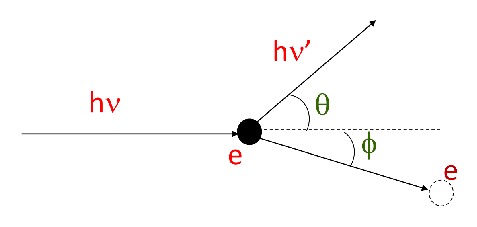
\includegraphics{compton}
		
		Coserving momenta in the $x$-direction,
		\begin{align*}
			\frac{h}{\lambda} &= \frac{h}{2\lambda}\cos\theta + p\cos\phi \\
			\therefore p\cos\phi &= \frac{h}{\lambda}
		\end{align*}
		Coserving momenta in the $y$-direction,
		\begin{align*}
			p\sin\phi &= \frac{h}{2\lambda}
		\end{align*}
		We, therfore have, $\tan\phi = 0.5$\\
		Therefore, $\phi = 26^{\circ}34'$
	\end{enumerate}
\end{document} 
